\scanpage{411}
\mspage{208}

and unless I am mistaken, it has become obvious
that this functor is an \uline{equivalence of
categories} (and as a consequence, there
\margin{\unsure{for the} \uline{\unsure{isomorphisms}}}
is the functor in the opposite direction :
drill holes at ``points'' invariant
under $\Gamma_{\unsure{a|0}}$ (or at arbitrary points,
at the cost of passing to a smaller $\Gamma'$).

But I realize that
\deleted{\illegible{1}} this is not at all obvious -- I am going
to try to elucidate the situation axiomatically.
We have fixed a genus $g$,
we suppose given, for varying $\nu$
(such that $(g,\nu)$ anabelian) closed
subgroups $N_{g,\nu}\subset\widehat{\widehat{\mathcal T}}_{g,\nu}$,
normalizing $\widehat{\mathcal T}_{g,\nu}$, and satisfying the
essential condition that the $\psi_i:\widehat{\widehat{\mathcal T}}_{g,\nu}\longrightarrow\widehat{\widehat{\unsure{\mathcal G|\mathcal S}}}_{g,\nu-1}$
induce
\[
M_{g,\nu}\xrightarrow{\sim}M_{g,\nu-1}
\]
Which makes it possible to define the notion
of arithmetization of a profinite $\pi$ of
anabelian type $(g,\nu)$, and the theory of

\scanpage{412}

plugging an arbitrary number of holes, and
of drilling just 1 hole, in the
category of groups of type $g,\nu$,
arithmetized.

We suppose on the other hand \unsure{given|given} a
full subcategory of the category of profinite
\margin{\unsure{we suppose it} : stable under taking open subgroups.}
groups (which could reduce to the
open subgroups of $\mathbb{\Gamma}_g$, common
value of the $\mathbb{\Gamma}_{g,\nu}$ or of open subgroups
of the group $\mathbb{\Gamma}_a$, $a$ an
arithmetization), and \deleted{some} \inserted{a notion of }outer operations
\inserted{``admissible''} of such $\Gamma$ on the
arithmetized $\pi$. We suppose

\textcircled{1} If $\Gamma$ operates admissibly on $\pi$, every
open subgroup too (\deleted{\unsure{and}} and conversely ?)

\textcircled{2} If moreover $\Gamma$ leaves invariant a subset $I'$
of $I=I(\pi)$, then by ``plugging $I'$'',
the operation of $\Gamma$ on $\pi'$ is admissible.

\margin{It suffices to \unsure{postulate it|prove it} for $\operatorname{card} I'=1$, i.e. plugging \unsure{a|a single} hole -- \unsure{at least if we know that the admissibility condition depends only on the action of the kernels of the groups}.}

\deleted{\illegible{1}}
\deleted{\unsure{We propose to define a notion of admissible action} \illegible{2}}
\inserted{When we have an \inserted{\uline{actual}} action, \unsure{(not outer)|(non-outer)}}
of $\Gamma$ on a $(\pi,a)$, then the functor
\unsure{of} ``\deleted{plugging}\inserted{drilling} holes'' gives an outer
action on a $(\pi^0,a^0)$ of type $g,\nu+1$,
and we say that the starting action is

\scanpage{413}
\mspage{209}

admissible, if the \uline{outer} action deduced is.

We thus find an \uline{equivalence} between
the category of \deleted{\unsure{categories}} systems $(\pi,a,\Gamma,\psi,i)$
of a $(\pi,a)$ of type $(g,\nu+1)$, with an
admissible \inserted{\uline{outer}} operation $\psi$ of a $\Gamma$ on it, and
an $i\in I(\pi)$ stable under $\Gamma$, with the category
of $(\pi',a',\Gamma,\psi')$ of $(\pi',a')$ of type
$(g,\nu)$, with a \uline{genuine} admissible action $\psi'$
of $\Gamma$ on it.

\deleted{\unsure{We must} \illegible{3}}
\inserted{Condition (1) ensures that}
\deleted{\textcircled{3} \unsure{If a genuine action}}
\inserted{if $\Gamma$ operates \deleted{\uline{\unsure{genuinely}}} \deleted{\unsure{admissible|admissibly}} actually, in a way}
admissible, then the outer action deduced
is admissible (but the converse will
not be true -- there will be ``pathological''
liftings of a given admissible \unsure{categorical|outer} action\ldots). We suppose moreover

\margin{\figure{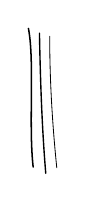
\begin{tikzpicture}[x=1cm,y=1cm,line cap=round,baseline=(current bounding box.center)]
\draw[line width=0.55pt] (0.04,1.80) .. controls (0.12,1.38) and (0.04,0.57) .. (0.10,0.04);
\draw[line width=0.50pt] (0.18,1.74) .. controls (0.19,1.20) and (0.21,0.55) .. (0.26,-0.04);
\draw[line width=0.30pt] (0.31,1.70) .. controls (0.31,1.09) and (0.35,0.52) .. (0.40,0.03);
\end{tikzpicture}}}
\textcircled{3} If $\Gamma$ operates \inserted{actually} in an admissible way on
$\pi$, then $\pi^\Gamma=(1)$.

\deleted{Let \unsure{Then}}
This implies that the category of
$\Gamma$-Points of $\pi$, or if you like of sections
of $B_{\pi,\Gamma}\,(\unsure{\simeq}B_u)$ over $B_\Gamma$, is \uline{rigid}.

\scanpage{414}

But \deleted{\unsure{let us call|let us suppose}} let us consider the inductive limit category of the \deleted{\illegible{1}} categories of sections of $B_{\pi,\Gamma}\simeq B_u$ over $B_{\Gamma'}$ ($\Gamma'$ an open subgroup), it is discrete and corresponds to the set
\[
\mathrm{Pt}_{\mathrm{ad}}(B_{\pi,\Gamma^{\natural}})\simeq
\underset{\substack{\Gamma'\ \mathrm{ouvert}\\\mathrm{de}\ \Gamma}}{\varinjlim}
\mathrm{Pt}_{\mathrm{ad}}(B_{\pi,\Gamma'}).
\]

\margin{\uline{N.B.} The groupoid with strict operators $\uline{\mathrm{Pt}}(B_{\pi,\Gamma})$ depends \unsure{functorially} on $(\pi,\Gamma)$, \illegible{1} for outer morphisms \deleted{\unsure{in}} \unsure{more} \illegible{3} of $\Gamma$, if \deleted{\illegible{4}}.}

\deleted{\textcircled{4} \unsure{For} \illegible{2} $\mathrm{Pt}(B_{\pi,\Gamma})$ \illegible{1}. On the other hand, $\pi$ can be defined by a groupoid.}
If $\mathrm{Pt}(B_{\pi,\Gamma})\ne\varnothing$, then (from the mere fact that $\pi^{\Gamma'}=(1)$ for $\forall$ open subgroup of $\unsure{\Gamma'|\Gamma}$) \inserted{the categorical group} $\pi$ can be described \unsure{canonically|commutatively} by a groupoid \inserted{profinite $\uline{\mathrm{Pt}}(B_{\pi,\Gamma^{\natural}})$} having $\mathrm{Pt}(B_{\pi,\Gamma})$ as object set, \deleted{\unsure{and|then}} \inserted{\unsure{linked|linked} by the categorical group $\pi$, on} which $\Gamma$ operates in the strict sense, with the stabilizer \inserted{$\Gamma_P$} of $\forall$ point being open. and $\Gamma_P\to\mathrm{Aut}(P)$ $(\simeq\pi\ \text{mod \unsure{inner automorphisms}})$

\deleted{More precisely, \unsure{independently of} the preceding axiomatics, we can describe the systems \unsure{formed} of a profinite group \inserted{categorical $\pi$}, and of an \inserted{outer} operation \unsure{of a profinite group} $\Gamma$ on it, \unsure{satisfying}}

being continuous. We have here \unsure{if} to $\forall\ P\in\mathrm{Pt}(B_{\pi,\Gamma})$ we associate the isomorphism class of \deleted{\unsure{groups of liftings}}

\scanpage{415}
\mspage{210}

\deleted{\unsure{groups}} of sections of $B_{\pi,\Gamma}$ over $B_\Gamma$, we find a bijection -- which characterizes the \inserted{$\Gamma$-}groupoid in question up to unique \uline{isomorphism}. We suppose

\textcircled{4} If $\Gamma$ operates admissibly on $(\pi,a)$, then there exists an open subgroup $\Gamma'$ of $\Gamma$ \deleted{can \unsure{operate in a way}} \inserted{whose \inserted{categorical} operation lifts to an} admissible actual operation -- i.e. $\mathrm{Pt}_{\mathrm{ad}}(B_{\Gamma,\pi})\ne\varnothing$.

\deleted{That said, let us consider \deleted{\illegible{1}} the situation of an admissible \inserted{outer} action of $\Gamma$ on $(\pi,a)$ and of an $i\in I(\pi)$ \deleted{stable} fixed under $\Gamma$. We thus have an \uline{actual} action \inserted{\unsure{admissible}} of $\Gamma$ on $(\pi',a')$, \deleted{and moreover we have} \inserted{thus an outer action,} plus a Point ``$\Gamma$-rational'', i.e. invariant under $\Gamma$. Let us consider on the other hand an admissible \unsure{lifting} $\Gamma\longrightarrow M(\pi,a)$, and \illegible{2}}

Let us note that in the situation envisaged, of plugging a hole $i\in I(\pi)$ of a $\pi$, in addition to the homomorphism
\[
\widehat{\widehat{\mathcal T}}(\pi)_i
\xrightarrow{\psi_i}
\widehat{\widehat{\unsure{\mathcal G|\mathcal S}}}(\pi'_i)
\]
associated, giving by composition
\[
\widehat{\widehat{\mathcal T}}(\pi)_i
\xrightarrow{\psi'_i}
\widehat{\widehat{\mathcal T}}(\pi'_i)
\]

\scanpage{416}

whence an outer action of $\widehat{\widehat{\mathcal T}}(\pi)$ on $\pi'_i$, \inserted{\unsure{in such a way} \unsure{that the} $\pi\overset{p_i}{\longrightarrow}\pi'_i$ \unsure{commute|commuting} with the outer actions of $\widehat{\widehat{\mathcal T}}(\pi)$, \deleted{\illegible{1}}} we have a canonical homomorphism of extensions, \deleted{associated} coming from this outer action and the homomorphism $p_i:\pi\longrightarrow\pi'_i$,

\diagram{\begin{tikzcd}[ampersand replacement=\&,column sep=2.4em,row sep=3.4em,
execute at end picture={
  \path (\tikzcdmatrixname-1-4.south west) -- (\tikzcdmatrixname-2-3.north east) coordinate[pos=.5] (lmfixnineteendiag);
  \draw[line width=.35pt] ([xshift=-5mm,yshift=1mm]lmfixnineteendiag) -- ([xshift=-6mm,yshift=1mm]lmfixnineteendiag) -- ([xshift=-6mm,yshift=-5mm]lmfixnineteendiag) -- ([xshift=-5mm,yshift=-5mm]lmfixnineteendiag);
  \draw[line width=.35pt] ([xshift=8mm,yshift=5mm]lmfixnineteendiag) -- ([xshift=9mm,yshift=5mm]lmfixnineteendiag) -- ([xshift=9mm,yshift=-1mm]lmfixnineteendiag) -- ([xshift=8mm,yshift=-1mm]lmfixnineteendiag);
}]
1 \arrow[r,dash] \& \pi \arrow[r,dash] \arrow[d,"p_i"] \&
\widehat{\widehat{\unsure{\mathcal G|\mathcal S}}}(\pi)_i \arrow[r] \arrow[d,"\varphi_i"] \&
\widehat{\widehat{\mathcal T}}(\pi)_i \arrow[r,dash] \arrow[d,"\psi'_i"] \arrow[dl,dashed,"\psi_i"'] \& 1 \\
1 \arrow[r,dash] \& \pi'_i \arrow[r] \&
\widehat{\widehat{\unsure{\mathcal G|\mathcal S}}}(\pi'_i) \arrow[r,dash] \&
\widehat{\widehat{\mathcal T}}(\pi'_i) \arrow[r,dash] \& 1
\end{tikzcd}}

which is not the \unsure{composite|composite}
\[
\widehat{\widehat{\unsure{\mathcal G|\mathcal S}}}(\pi)_i
\longrightarrow\widehat{\widehat{\mathcal T}}(\pi)_i
\xrightarrow{\psi_i}\widehat{\widehat{\unsure{\mathcal G|\mathcal S}}}(\pi'_i).
\]
(it can be defined whenever we have a group $\Gamma$, here $\widehat{\widehat{\mathcal T}}(\pi)$, which \deleted{\unsure{with trivial center}} \inserted{\unsure{commuting|commutes}} as outer actions on two outer groups $\pi,\pi'$, and we have a homomorphism \inserted{$\unsure{\beta|p}$} \deleted{\illegible{1}} $\pi\longrightarrow\pi'$ which commutes with the action of $\Gamma$, and such that the \inserted{center of $\pi$ and \unsure{the|the}} \unsure{centralizer|centralizers} of \unsure{its image|$\beta(\pi)$} in $\pi'$ are trivial\ldots)
\inserted{\unsure{This is also here} the ``transport of structure'' homomorphism}, \inserted{which} \unsure{for} \unsure{every|\deleted{every}} loop automorphism $u$ of $\pi$, associates the \unsure{corresponding|canonical} automorphism of $\pi'_i$.

We \unsure{have\deleted{vait}|\deleted{had}} forgotten to specify:

\textcircled{\unsure{g|9}} The canonical homomorphism $(\widehat{\widehat{\unsure{\mathcal G|\mathcal S}}}_{g,\nu})_i\longrightarrow\widehat{\widehat{\unsure{\mathcal G|\mathcal S}}}_{g,\nu-1}$ associated with $i\in[0,\nu-1]$, sends $(M_{g,\nu})_i$ into $M_{g,\nu-1}$ \deleted{into} so it fits into a \unsure{homomorphism|diagram} of exact sequences

\scanpage{417}
\mspage{211}

\begin{samepage}
(26)
\diagram{
\begin{tikzcd}[ampersand replacement=\&,row sep=6em]
1 \arrow[r,dash] \& \pi \arrow[r,dash] \arrow[d] \&
M_a(\pi)_i \arrow[r] \arrow[d, "\varphi_i"']
\arrow[dr, phantom, "{\text{\shortstack{\unsure{\uline{not}|\uline{not}}\\\unsure{commutative?}}}}" description, near start] \&[65pt]
N_a(\pi)_i \arrow[r] \arrow[d, "\text{\unsure{commutative}}"',pos=.75] \arrow[dl, dashed] \& 1 \\
1 \arrow[r,dash] \& \pi'_i \arrow[r] \&
M_{a'}(\pi'_i) \arrow[r,dash] \& N_{a'}(\pi'_i) \arrow[r,dash] \& 1
\end{tikzcd}
\par [The horizontal segments issuing from the two $1$ on the left have no visible arrowhead. The right ends of the segments $\pi$--$M_a(\pi)_i$ at the top, $M_{a'}(\pi'_i)$--$N_{a'}(\pi'_i)$ and $N_{a'}(\pi'_i)$--$1$ at the bottom are thickened, with no arrowhead legible with certainty. An ink blot (overwriting) follows the parenthesis of $M_a(\pi)_i$. The word \unsure{commutative} is written in the right-hand triangle, between the dotted arrow and the right-hand vertical arrow; it is not a legible label of the dotted arrow.]
}
\end{samepage}.

This being so, if we have an admissible \inserted{outer} operation
$\Gamma\longrightarrow N_a(\pi)$ of $\Gamma$ on $\pi$,
\inserted{fixing $i$,} hence also through
$N_a(\pi)\longrightarrow N_{a'}(\pi'_i)$ on $\pi'_i$,
we can consider that \unsure{\deleted{every}} lifting
$\Gamma\longrightarrow M_a(\pi)$ \inserted{for $\pi$} defines
by composition a lifting $\Gamma\longrightarrow M_{a'}(\pi'_i)$
for $\pi'_i$. \deleted{To say that}
\inserted{We easily conclude from}
\textcircled{2} that if the first is admissible, the second is.
We thus find
\[
(27)\qquad
\mathrm{Pt}_{\mathrm{ad}}(B_{\pi,\Gamma})
\longrightarrow
\mathrm{Pt}_{\mathrm{ad}}(B_{\pi'_i,\Gamma})
\]
(and passing to the limit, a map of $\Gamma$-sets
\[
(28)\qquad
\mathrm{Pt}_{\mathrm{ad}}(B_{\pi,\Gamma^{\natural}})
\longrightarrow
\mathrm{Pt}_{\mathrm{ad}}(B_{\pi'_i,\Gamma^{\natural}})
\]
-- which moreover corresponds to a homomorphism of \unsure{$\Gamma$} groupoids
\[
(29)\qquad
\uline{\mathrm{Pt}}_{\mathrm{ad}}(B_{\pi,\Gamma^{\natural}})
\longrightarrow
\uline{\mathrm{Pt}}_{\mathrm{ad}}(B_{\pi'_i,\Gamma^{\natural}}).
\]

This being so, let $P\in\mathrm{Pt}_{\mathrm{ad}}(B_{\pi'_i,\Gamma})$
be the ``canonical point'' of
$\mathrm{Pt}_{\mathrm{ad}}B_{\pi'_i,\Gamma}
=\bigl(\mathrm{Pt}_{\mathrm{ad}}(B_{\pi'_i,\Gamma^{\natural}})\bigr)^\Gamma$.

\scanpage{418}

We ask:

\textcircled{5} The map (27) induces a \uline{bijection}\unsure{.}
\figure{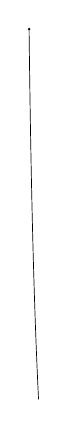
\begin{tikzpicture}[x=1mm,y=1mm,baseline=(current bounding box.north)]
\fill (0,0) circle[radius=.18mm];
\draw[line width=.25pt,line cap=round] (0,-.2) .. controls (.15,-13) and (.45,-32) .. (1.2,-47);
\end{tikzpicture}}
\[
\mathrm{Pt}_{\mathrm{ad}}(B_{\pi,\Gamma})
\longrightarrow
\mathrm{Pt}_{\mathrm{ad}}(B_{\pi'_i,\Gamma})\setminus\{P\}
\]
or again (passing to the limit) a bijection of $\Gamma$-sets
\[
\mathrm{Pt}_{\mathrm{ad}}(B_{\pi,\Gamma^{\natural}})
\simeq
\mathrm{Pt}_{\mathrm{ad}}(B_{\pi'_i,\Gamma^{\natural}})\setminus\{P\}
\]

This means three things:

a) The canonical homomorphism $\Gamma\longrightarrow M_{a'}(\pi'_i)$,
the composite of $\Gamma\longrightarrow N_a(\pi)$ and
$N_a(\pi)\simeq M_{a'}(\pi'_i)$,
is not \inserted{$\pi'_i$-}conjugate to a composite homomorphism
$\Gamma\xrightarrow{\lambda}M_a(\pi)
\xrightarrow{\varphi_i}M_{a'}(\pi'_i)$,
where $\Gamma\xrightarrow{\lambda}M_a(\pi)$ is an admissible lifting.

b) If $\lambda,\mu:\Gamma\rightrightarrows M_a(\pi)$ are two
admissible liftings of $\Gamma\longrightarrow N_a(\pi)$
\deleted{\unsure{that}} such that
$\varphi_i\circ\lambda$ and $\varphi_i\circ\mu:
\Gamma\rightrightarrows M_a(\pi)$ are
\inserted{$\pi'_i$-}conjugate, then $\lambda$ and $\mu$ are already
\inserted{$\pi$-}conjugate.

c) Every admissible lifting of
$\Gamma\longrightarrow N_{a'}(\pi'_i)$ to
$\Gamma\longrightarrow M_{a'}(\pi'_i)$,
comes by composition from an admissible lifting
$\Gamma\longrightarrow M_a(\pi)$.

\scanpage{419}
\mspage{212}

Thanks to this, the equivalence of categories between systems
$(\pi,a,i,\Gamma,\unsure{\theta}:\Gamma\mathop{\longrightarrow}\limits_{\unsure{\mathrm{adm}}}\unsure{N_a})$,
and the systems $(\pi',a',\Gamma,\theta':\Gamma\longrightarrow\unsure{N_{a'}},P)$,
where $P\in\mathrm{Pt}(B_{\pi',\Gamma^{\natural}})^\Gamma$,
becomes perfectly precise at the level of points: the
$\Gamma$-rational Points of $B_{\pi\unsure{,\Gamma^{\natural}|\deleted{,\Gamma^{\natural}}}}$
are identified with \unsure{one|the set}
\deleted{of the $\Gamma$-\unsure{rational} points} of the $\Gamma$-rational points
of $B_{\pi'}$, distinct from $P$.

This then allows us (which was not feasible in the discrete
context!) to extend the equivalence of categories to an equivalence

\[
\begin{gathered}(30)\\[3pt]
\begin{array}{c@{\,}c@{\,}c}
\parbox[t]{0.44\linewidth}{%
category of systems $(\pi,\unsure{a|\alpha},I',\allowbreak\Gamma,\allowbreak\theta:\Gamma\longrightarrow N_a)$
of an arithmetized $\pi$ \inserted{(by \unsure{$\alpha$|$a$})} of type $(g,\nu)$,
of $I'\subset I(\pi)$, of an
\uline{admissible} outer action of $\Gamma$ on $\pi$
such that $\Gamma$ \deleted{\unsure{operates}} \uline{fixes each point} of $I'$
}
& \unsure{\cong|\simeq} &
\parbox[t]{0.44\linewidth}{%
category of systems
$(\pi',\unsure{a'|\alpha'},I',\allowbreak\unsure{\Gamma^{*}|\Gamma},\allowbreak\theta':\Gamma\longrightarrow N_{a'})$
of an arithmetized $\pi'$ (by \unsure{$a'$|$\alpha'$}) of type
$(g,\nu')$ $[\nu'=\nu-\mathrm{card}(I')]$
with an admissible \inserted{outer} operation of $\Gamma$ on it, and
a subset $I'\subset\mathrm{Pt}_{ad}(B_{\pi',\unsure{\Gamma}}\unsure{)}$
(hence $I'\subset\mathrm{Pt}_{ad}(B_{\pi',\Gamma})^\Gamma$)
i.e. $I'$ formed of points \unsure{invariant|fixed} under $\Gamma$, i.e. ``$\Gamma$-rational''
}
\end{array}
\end{gathered}\]

\margin{with $2g+(\underbrace{\nu-\mathrm{card}\,I'}_{\nu'})\geq3$}

We thus have a quasi-inverse functor:
drilling holes at $I'$ !

\scanpage{420}

It is to be noted that in this approach, we have had to restrict ourselves to the case
\deleted{\unsure{of the|of}} \inserted{of a set of} points \deleted{\illegible{1}}
$I'\subset I(\pi)$ not only stable under $\Gamma$, but
\deleted{\unsure{formed}} $\subset I^\Gamma$
\deleted{fixed under $\Gamma$} or again to a subset
$I'\subset\mathrm{Pt}(B_{\pi',\Gamma^{\natural}})$
not only stable under $\Gamma$, but
\unsure{even|=}\,$\subset\mathrm{Pt}(B_{\pi',\Gamma^{\natural}})^\Gamma$.
To show that without this restriction, the natural functor
\deleted{\unsure{is}} that corresponds is nevertheless
an equivalence, we are reduced to this

\textcircled{6} Let $(\pi,a,I'\subset I(\pi))$ be with $(\pi,a)$
an arithmetized \inserted{categorical} \unsure{profinite|profinite} group with loops of type
$g,\nu$, whence $(\pi',a')$ --- let $\Gamma$ be, with $\Gamma'$
an open subgroup operating on $(\pi,a)$ in an admissible way
$(\Gamma\longrightarrow N_a(\pi))$,
and leaving $I'$ stable, hence it operates in an admissible way on
$(\pi',a')$,
Suppose given a \uline{lifting} of this action of $\Gamma'$
to an admissible action of $\Gamma$ on $N_{a'}$, which leaves invariant
\[
\begin{array}{rcl}
I'&\subset&\mathrm{Pt}(B_{\pi',\Gamma^{\natural}}).\\
&&\rotatebox{90}{$\unsure{\simeq}$}\\
&&\mathrm{Pt}(B_{\pi',\Gamma^{\prime\natural}})
\end{array}
\]

\diagram{\begin{tikzcd}[ampersand replacement=\&,column sep=3.6em,row sep=3em]
{\deleted{\unsure{M_a}}\;(N_a)_{I'}} \arrow[d] \&
\Gamma' \arrow[l] \arrow[d,hook,line width=.9pt] \arrow[dl,bend right=7,line width=.65pt] \\
N_{a'} \& \Gamma \arrow[l] \arrow[ul,dashed]
\end{tikzcd}}

Then there exists a unique admissible action of $\unsure{\Gamma|\Gamma'}$
on $(\pi,a)$, which extends that of $\Gamma'$ and which gives rise
to the \inserted{given} one on $\pi'$.
